\documentclass[aspectratio=169]{beamer}

\usetheme{Boadilla}
\usecolortheme{dolphin}
\setbeamertemplate{navigation symbols}{}
\setbeamertemplate{footline}[frame number]

\usepackage{amsmath,amssymb}
\usepackage{graphicx}

\graphicspath{
  {../../output/model/}
  {../../output/graphs/}
  {../../output/graphs/model/}
  {output/model/}
  {output/graphs/}
  {output/graphs/model/}
}

\title[AI \& Labor Market Risk]{Present Day, Present Time:\\
  AI Exposure \& Labor Market Risk}
\author{Leyao Wang}
\institute{University of Virginia \\ ECON 4210 --- International Trade}
\date{March 2026}

\definecolor{myred}{RGB}{215,48,39}
\definecolor{mygreen}{RGB}{26,150,65}
\definecolor{mygray}{RGB}{120,120,120}

\begin{document}

\begin{frame}
\titlepage
\end{frame}

% =============================================================================
% SLIDE 2 — Motivation
% =============================================================================
\begin{frame}{The Question}

\begin{columns}[c]
\column{0.55\textwidth}

  \textbf{November 2022: ChatGPT launches.}\\[10pt]

  Millions of people start using AI to do things that \emph{people get paid to do}.

  \bigskip
  \textbf{Some workers are much more exposed than others.}

  \bigskip
  \large\textbf{Did it cost them?}

\column{0.42\textwidth}
  \centering
  
\includegraphics[width=0.85\linewidth]{toy_model.png}\\
  {\small\color{mygray} Workers differ in how substitutable their tasks are}

\end{columns}

\end{frame}

% =============================================================================
% SLIDE 3 — Trade theory intuition
% =============================================================================
\begin{frame}{A Lesson from Trade Economics}

\textbf{Offshoring (2000s):} companies shipped tasks abroad when foreign labor was cheaper

\bigskip
\begin{itemize}
  \item \textbf{Grossman \& Rossi-Hansberg (2008):} it's not whole jobs that get offshored ---
  it's specific \emph{tasks}

  \bigskip
  \item \textbf{Ottaviano, Peri \& Wright (2013):} different workers face different cutoffs ---
  not everyone equally at risk

  \bigskip
  \item \textbf{AI is the same story, new technology:}\\[4pt]
    Instead of cheap foreign workers --- a cheap \emph{machine}.\\
    \textbf{``Offshoring'' your tasks to Claudeland, GPTopia, Geminia\ldots}
\end{itemize}

\end{frame}

% =============================================================================
% SLIDE 4 — The Model
% =============================================================================
\begin{frame}{The Model: AI as a Supply Shock}

\textbf{Key idea:} AI doesn't set prices --- it \emph{adds supply} to the tasks it can do

\medskip
\begin{columns}[c]
\column{0.52\textwidth}
  
\includegraphics[width=\linewidth]{fig_postai.png}
\column{0.45\textwidth}
  \small
  \begin{itemize}
    \item Every task has human supply $f(i)$.
          AI adds $s(i)$ on top --- but only below $I^*$

    \medskip
    \item \textbf{Left of $I^*$:} more supply $\rightarrow$ wages fall
    \begin{itemize}
      \item[\textcolor{myred}{$\rightarrow$}] \textcolor{myred}{wage compression}
    \end{itemize}

    \medskip
    \item \textbf{Right of $I^*$:} no AI supply, but the
          economy grew $\rightarrow$ wages rise

    \medskip
    \item As AI improves, $I^*$ shifts right
  \end{itemize}
\end{columns}

\end{frame}

% =============================================================================
% SLIDE 5 — Prediction
% =============================================================================
\begin{frame}{What the Model Predicts}

\textbf{Workers to the left of $I^*$ face two pressures:}

\bigskip
\begin{columns}[t]
\column{0.48\textwidth}
  \textbf{\textcolor{myred}{Wage compression}}\\[6pt]
  AI floods their task market with supply $\rightarrow$ their scarcity falls $\rightarrow$ lower pay

\column{0.48\textwidth}
  \textbf{\textcolor{myred}{Displacement}}\\[6pt]
  If the compressed wage drops below what you're willing to accept $\rightarrow$ you exit

\end{columns}

\bigskip\hrule\bigskip

{\small\color{mygray}
\textit{One channel is set aside: \textbf{augmentation} --- AI may eventually raise productivity
of workers it complements rather than supplements. Left for future work.}}

\end{frame}

% =============================================================================
% SLIDE 6 — The Strategy
% =============================================================================
\begin{frame}{The Strategy}

\begin{columns}[c]
\column{0.54\textwidth}
  \[
    Y_{it} = \alpha + \!\!\sum_{t \neq 2022}\!\! \beta_t \bigl(\mathbf{1}[t] \times \mathrm{AIExp}_i\bigr)
    + X_{it}'\Gamma + \varepsilon_{it}
  \]
  {\small\color{mygray}
    $X_{it}$: sex, education, state$\times$year FEs\\
    SEs clustered by occupation \quad Baseline: 2022 $(\beta_{2022} \equiv 0)$
  }

\column{0.43\textwidth}
  \small
  \begin{itemize}
    \item \textbf{Data:} CPS, 500K+ data points, 2018--2025
    \item \textbf{AI exposure:} Eloundou et al.\ (2024), occupation-level LLM score
    \item \textbf{Strategy:} high vs.\ low exposure, before vs.\ after ChatGPT
    \item \textbf{Model says:} $\beta_t$ diverges post-2022
  \end{itemize}
\end{columns}

\end{frame}

% =============================================================================
% SLIDE 7 — Unemployment Results
% =============================================================================
\begin{frame}{Result 1: Unemployment}

\begin{columns}[c]
\column{0.62\textwidth}
  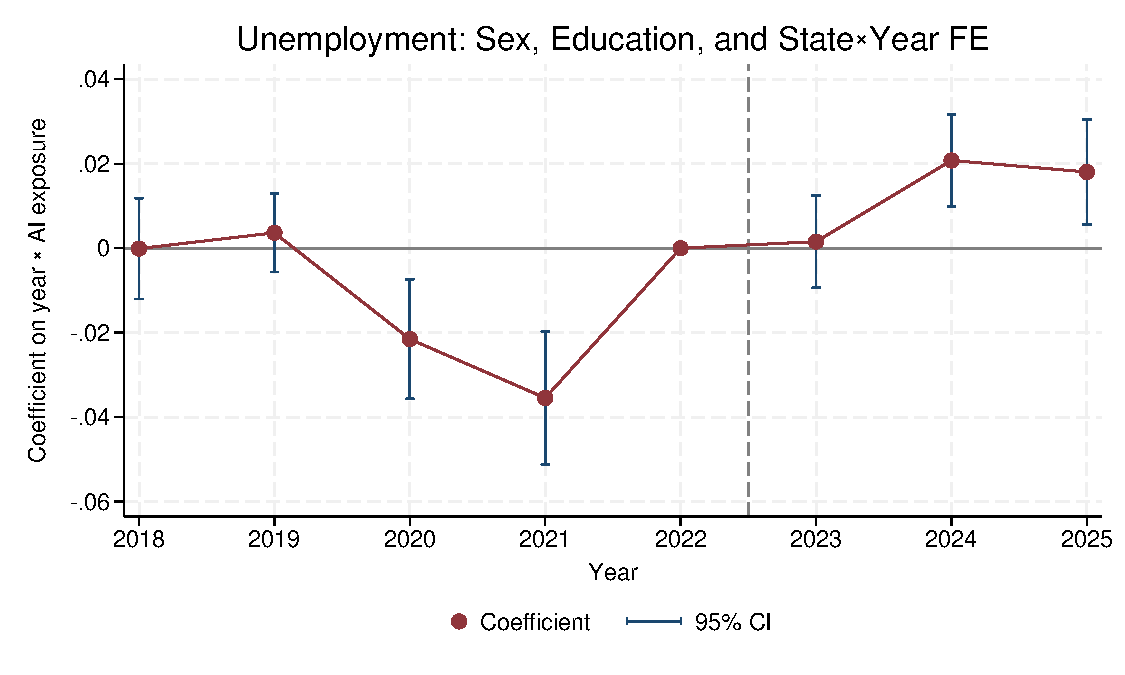
\includegraphics[width=\linewidth]{unemployment_stateYFE_plot.pdf}
\column{0.35\textwidth}
  \small
  \begin{itemize}
    \item \textcolor{red}{\textit{Interesting}} pre-trends before 2022 --- what happened in 2020
    \medskip
    \item \textbf{Post-2022:} high-exposure workers show a rising unemployment gap
    \medskip
    \item Effect holds across all specifications
  \end{itemize}
\end{columns}

\end{frame}

% =============================================================================
% SLIDE 8 — Wage Results
% =============================================================================
\begin{frame}{Result 2: Wages}

\begin{columns}[c]
\column{0.62\textwidth}
  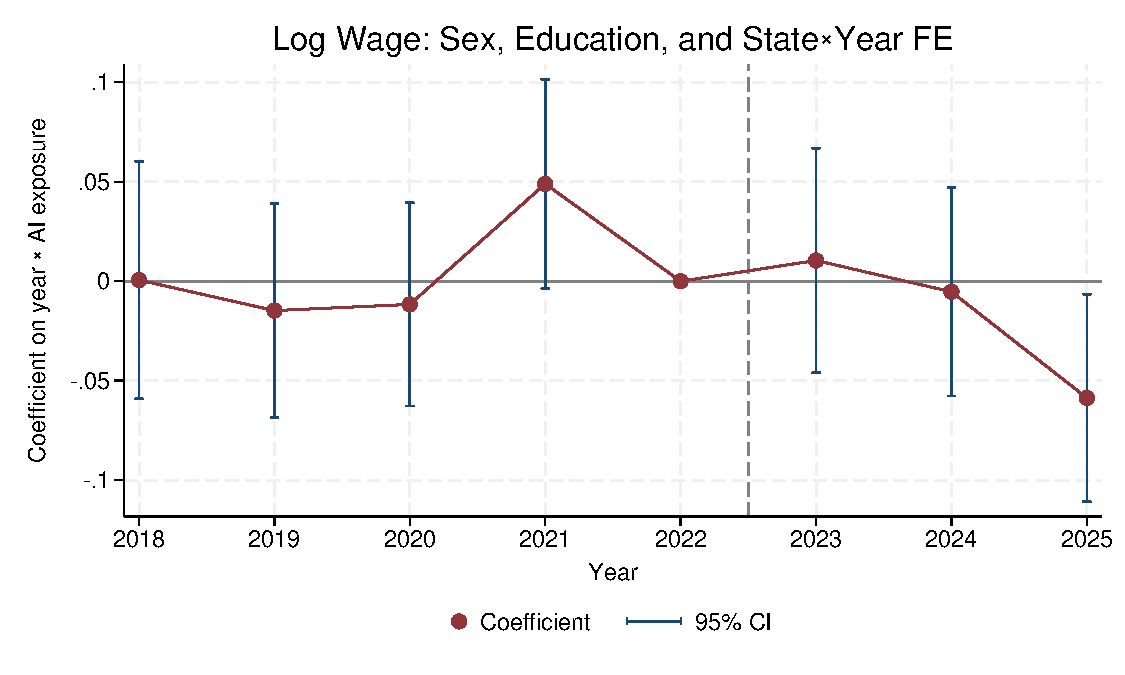
\includegraphics[width=\linewidth]{logwage_stateYFE_plot.pdf}
\column{0.35\textwidth}
  \small
  \begin{itemize}
    \item Flat pre-trends --- consistent baseline
    \medskip
    \item \textbf{Post-2022:} wages compress for high-exposure workers
    \medskip
    \item Non-college workers bear the brunt
  \end{itemize}
\end{columns}

\end{frame}

% =============================================================================
% THANK YOU
% =============================================================================
\begin{frame}{}
\centering
\vspace{1.5cm}
{\Large Thank you!}\\[1cm]
{\normalsize Questions welcome.}\\[1.5cm]
\begin{columns}[c]
\column{0.45\textwidth}
  \centering
  {\small\color{mygray} \textit{Bottom line:}\\[4pt]}
  {\normalsize AI is like offshoring ---\\
  some workers face immediate\\
  wage and employment risk}
\column{0.45\textwidth}
  \centering
  {\small\color{mygray} \textit{The data says:}\\[4pt]}
  {\normalsize Yes, high-exposure workers\\
  are already seeing it ---\\
  unemployment \emph{and} potentially wages}
\end{columns}
\end{frame}

% =============================================================================
% BACKUP SLIDES
% =============================================================================
\appendix

\begin{frame}{}
\centering
\vspace{2cm}
{\large\color{mygray} \textit{Backup: The Dirty Work}}\\[0.5cm]
{\small\color{mygray} Formal model, derivations, and further discussion of $I^*$}
\end{frame}

% --- B1: Model Setup ---
\begin{frame}{Model Setup (Formal)}

\begin{itemize}
  \item \textbf{Tasks} indexed $i \in [0,1]$ by AI susceptibility
  \begin{itemize}
    \item Low $i$: routine cognitive --- easy for AI \quad|\quad High $i$: complex --- hard for AI \textit{currently}
  \end{itemize}

  \medskip
  \item \textbf{CES Production}:
  \[
    Y = \left[\int_0^1 y(i)^{\frac{\sigma-1}{\sigma}}\,di\right]^{\!\frac{\sigma}{\sigma-1}}
  \]

  \medskip
  \item \textbf{Workers:} type $i^*$ specializes in task $i^*$; supply of task $i$ is $f(i)$ (fixed, inelastic)

  \medskip
  \item \textbf{AI supply} of task $i$: $\quad s(i) \geq 0,\;$ $s'(i)<0$ for $i<I^*$, $\;s(i)=0$ for $i\geq I^*$
  \begin{itemize}
    \item AI adds to supply of routine tasks; $I^*$ is the capability frontier
  \end{itemize}

  \medskip
  \item Competitive firms; output price $P_Y$ fixed (small open economy)
\end{itemize}

\end{frame}

% --- B2: Pre-AI Derivation ---
\begin{frame}{Pre-AI Equilibrium: Derivation}

\textbf{Firm cost minimization gives task demand:}
\[
  y^d(i) \;=\; Y \cdot \left(\frac{P_Y}{p_0(i)}\right)^{\!\sigma}
\]

\textbf{Market clearing} $\bigl(y^d(i) = f(i)\bigr)$ pins down task price:
\[
  p_0(i) \;=\; P_Y \cdot \left(\frac{Y}{f(i)}\right)^{\!1/\sigma}
\]

\textbf{Solve for $Y_0$} --- plug $y(i)=f(i)$ back into the CES aggregator:
\[
  \boxed{Y_0 \;=\; \left[\int_0^1 f(i)^{\frac{\sigma-1}{\sigma}}\,di\right]^{\!\frac{\sigma}{\sigma-1}}}
\]

\begin{itemize}
  \item $Y_0$ is fully determined by worker distribution $f$ --- not by prices
\end{itemize}

\end{frame}

% --- B3: Pre-AI Wage Schedule ---
\begin{frame}{Pre-AI Equilibrium: Wage Schedule}

Under full specialization, each worker earns their task price:
\[
  w_0(i^*) \;=\; p_0(i^*) \;=\; P_Y \cdot \left(\frac{Y_0}{f(i^*)}\right)^{\!1/\sigma}
\]

\centering
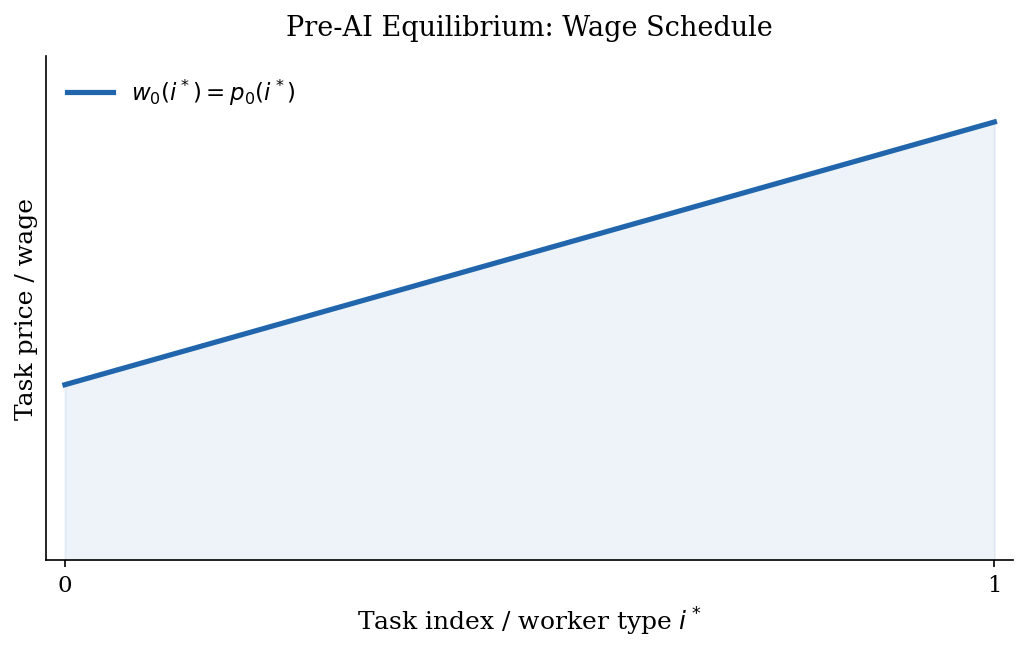
\includegraphics[width=0.72\linewidth]{fig_preai.png}

{\small\itshape Supply $f(i)$ is downward-sloping (more workers in routine tasks);
wage $w_0$ mirrors it upward (scarcer tasks pay more).}

\end{frame}

% --- B4: Post-AI Supply Shock ---
\begin{frame}{Post-AI: The Supply Shock}

AI adds supply $s(i)$ to tasks below $I^*$. Effective supply becomes $\bar y(i)=f(i)+s(i)$.

\medskip
New output: $\;\bar Y = \bigl[\int_0^1 \bar y(i)^{(\sigma-1)/\sigma}\,di\bigr]^{\sigma/(\sigma-1)} > Y_0$

\medskip
Post-AI wage (same CES logic):
\[
  \boxed{w_1(i^*) \;=\; P_Y\!\left(\frac{\bar Y}{f(i^*)+s(i^*)}\right)^{\!1/\sigma}}
\]

\medskip
\begin{itemize}
  \item \textbf{Numerator} $\bar Y > Y_0$: economy grew $\rightarrow$ pushes wages \textcolor{mygreen}{up}
  \item \textbf{Denominator} $f+s > f$ for $i<I^*$: more supply $\rightarrow$ pushes wages \textcolor{myred}{down}
  \item For $i\geq I^*$: $s=0$, only numerator moved $\rightarrow$ wages \textcolor{mygreen}{rise}
  \item For $i<I^*$: denominator growth outpaces numerator for heavily exposed workers $\rightarrow$ wages \textcolor{myred}{fall}
\end{itemize}

\smallskip
{\small\color{mygray} One channel set aside: \emph{augmentation} (AI raising worker productivity). Left for future work.}

\end{frame}

% --- B5: Post-AI Figures ---
\begin{frame}{Post-AI: Two Scenarios}

\centering

\includegraphics[width=0.82\linewidth]{fig_postai.png}

\smallskip
{\small Moderate AI supply: mild compression.  Heavy AI supply: deep compression below $I^*$,
larger gains above.  The outcome depends on the magnitude of $s(i)$ relative to $f(i)$.}

\end{frame}

% --- B6: Expanding Frontier + Non-Monotone f ---
\begin{frame}{Further Discussion of $I^*$}

\begin{columns}[t]
\column{0.50\textwidth}

  \textbf{As AI improves, $I^*$ shifts right}\\[4pt]
  More workers exposed, deeper compression.

  \medskip
  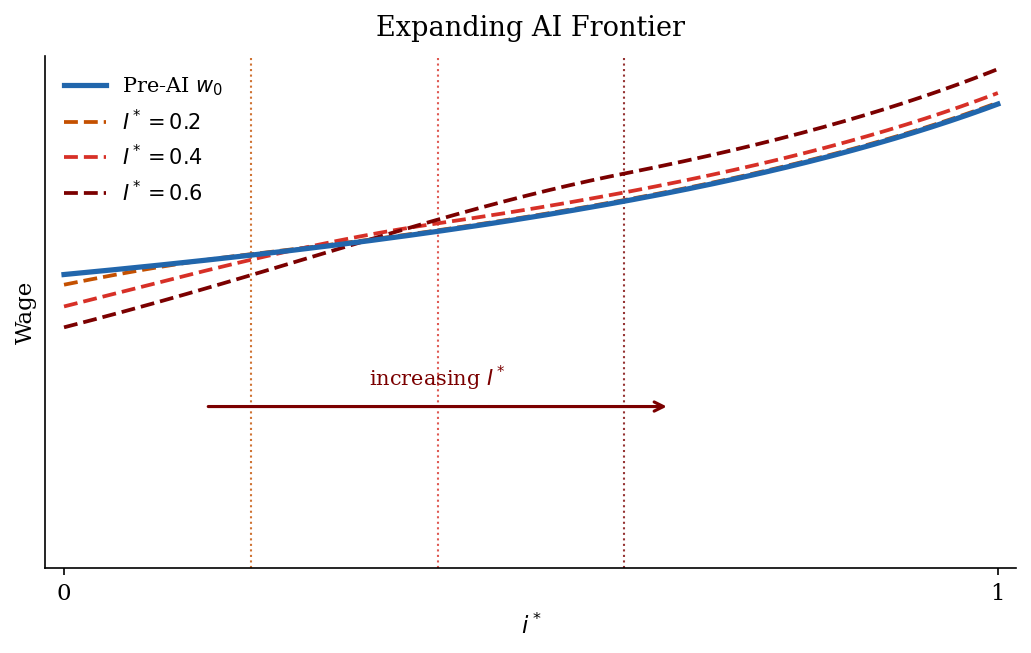
\includegraphics[width=\linewidth]{fig_capability.png}
  {\tiny Each curve shows $w_1$ for a different $I^*$. Higher $I^* \rightarrow$ wider compression.}

\column{0.48\textwidth}

  \textbf{Non-monotone $f(i)$: scattered effects}\\[4pt]
  If many workers cluster in a mid-complexity task, wage compression need not be contiguous.

  \medskip
  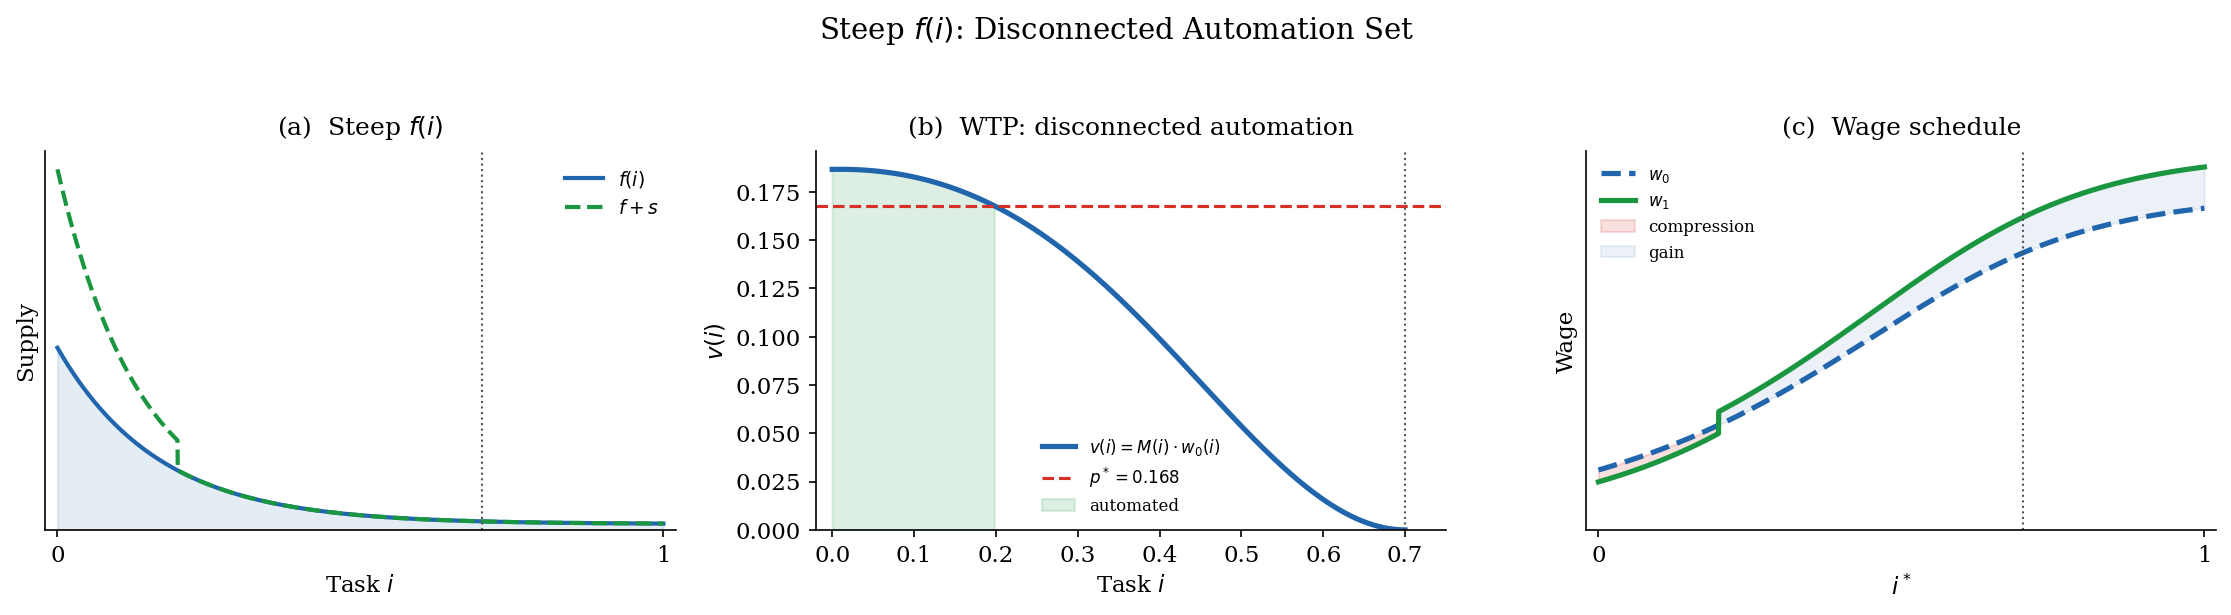
\includegraphics[width=\linewidth]{fig_multiple.png}
  {\tiny Bump in $f$ near $i\approx 0.55$ creates a local dip in $w_0$ and a pocket where workers may gain even inside $[0,I^*)$.}

\end{columns}

\end{frame}

\end{document}
